\chapter{Egy frekvenciaváltó tervezése}

\paragraph{}
A frekvenciaváltó egy olyan eszköz mely váltakozó áramú bemenetből váltakozó áramú kimenetet állít elő, mint ahogy a neve is mutatja, más frekvenciával vagy akár feszültséggel, mint a bemenet. Erre azért van szükség, mert a meghajtani kívánt folyamatnak nagyon valószínű, hogy más igényei vannak, mint amit a hálózat önmagában képes biztosítani. Értem ez alatt azt, hogy közvetlen összeköttetés esetén a motorunk $50\ Hz-el$, vagy ennek egész számú hányadosával tudna forogni, illetve ennek a paraméter a befolyásolása fizikailag csak a motor módosításával lehetséges. Természetesen mint az ipar és az élet minden szegmensében itt is célunk a feladat minél hatékonyabb végrehajtása. A világon a teljes villamosenergia felhasználás mint egy $25\ \%-$-át adják a villamos hajtások és ez a szám folyamatosan nő (pl. az elektromos közlekedés térnyerésével). Az igény tehát nyilvánvaló ezeknek az eszközöknek a folyamatos fejlesztésére.

\begin{figure}[!h]
	\centering
	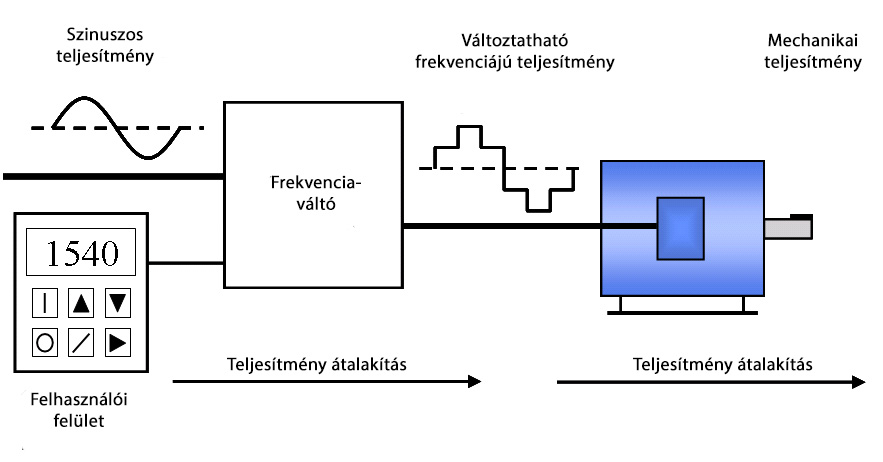
\includegraphics[width = \textwidth]{figures/VFD_System.jpg}
	\caption{A frekvenciaváltó szerepe} 
	\label{fig:vfd_system}
\end{figure}

\paragraph{}
A korábban az ilyen teljesítmény átalakítási feladatokat elektromechanikus berendezésekkel oldották meg, nevezetesen egy motor és generátor párral, ahol is a megfelelő póluspár arány kiválasztásával a frekvenciát módosítani lehetett. Amennyiben szükséges volt feszültségmódosítás is, megfelelő áttételű transzformátor segítségével valósították meg. Ezt követően megjelentek a vákumcsöves eszközök, azonban az igazi áttörést a teljesítményelektronikai félvezető elemek megjelenése okozta. 

\section{Az eszköz felépítése}



\section{A szükséges kompetenciák}
\section{A fejlesztés folyamata}
